\documentclass[12pt]{article}
\usepackage{pgfplots, url, tikz, graphicx}
\usepackage{enumitem} % To customize enumerate
\usepackage{amssymb}
\usepackage{caption}
\usepackage{subcaption}
\usepackage{amsmath}
\usepackage{float}
\usepackage{sagetex}

\usetikzlibrary{arrows.meta, positioning}
\pgfplotsset{compat=1.18}

\title{Math HW Week 8}
\author{Duc Nguyen}
\date{\today}

\begin{document}
\maketitle
\section*{Applied Math}
\subsection*{\#2}
\begin{enumerate}[label=\alph*.]
    \item 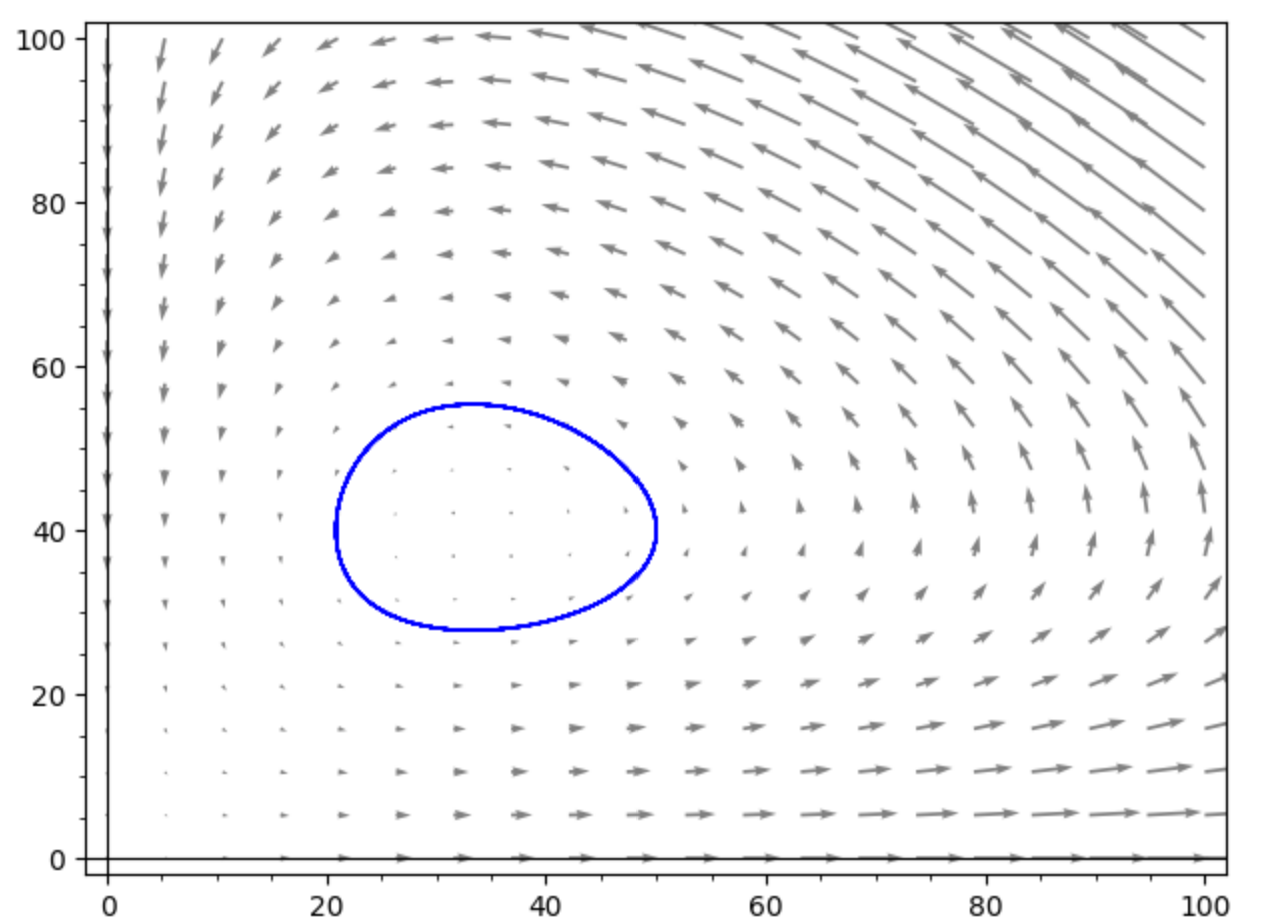
\includegraphics[width=0.5\textwidth]{hw8.png}
    \item 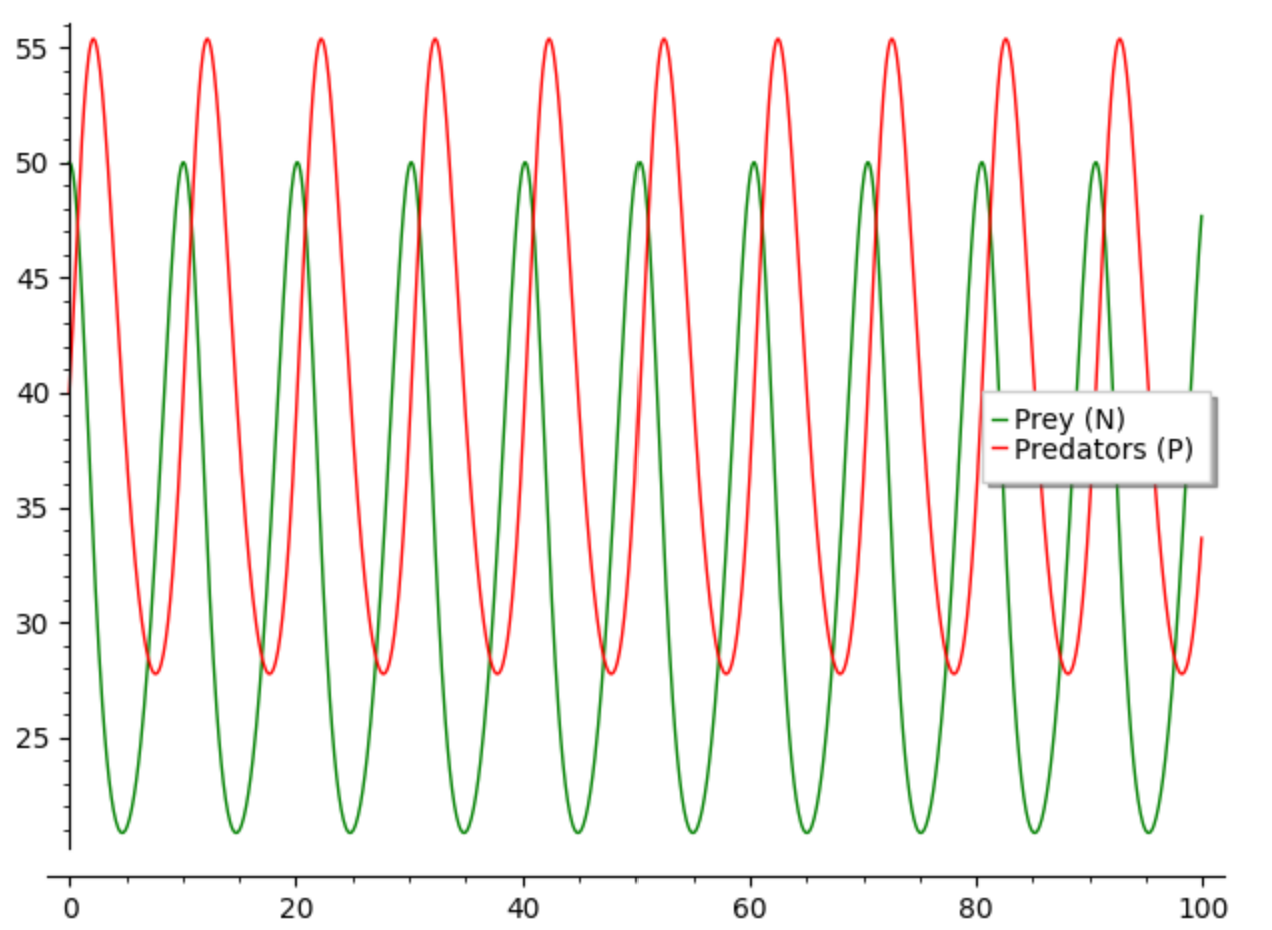
\includegraphics[width=0.5\textwidth]{hw8_2.png}

\item There would be a total of around 56 predators, with 34 prey at that time
\item If there are 74 predators, 20\% of them got removed means there are 59 predators left.

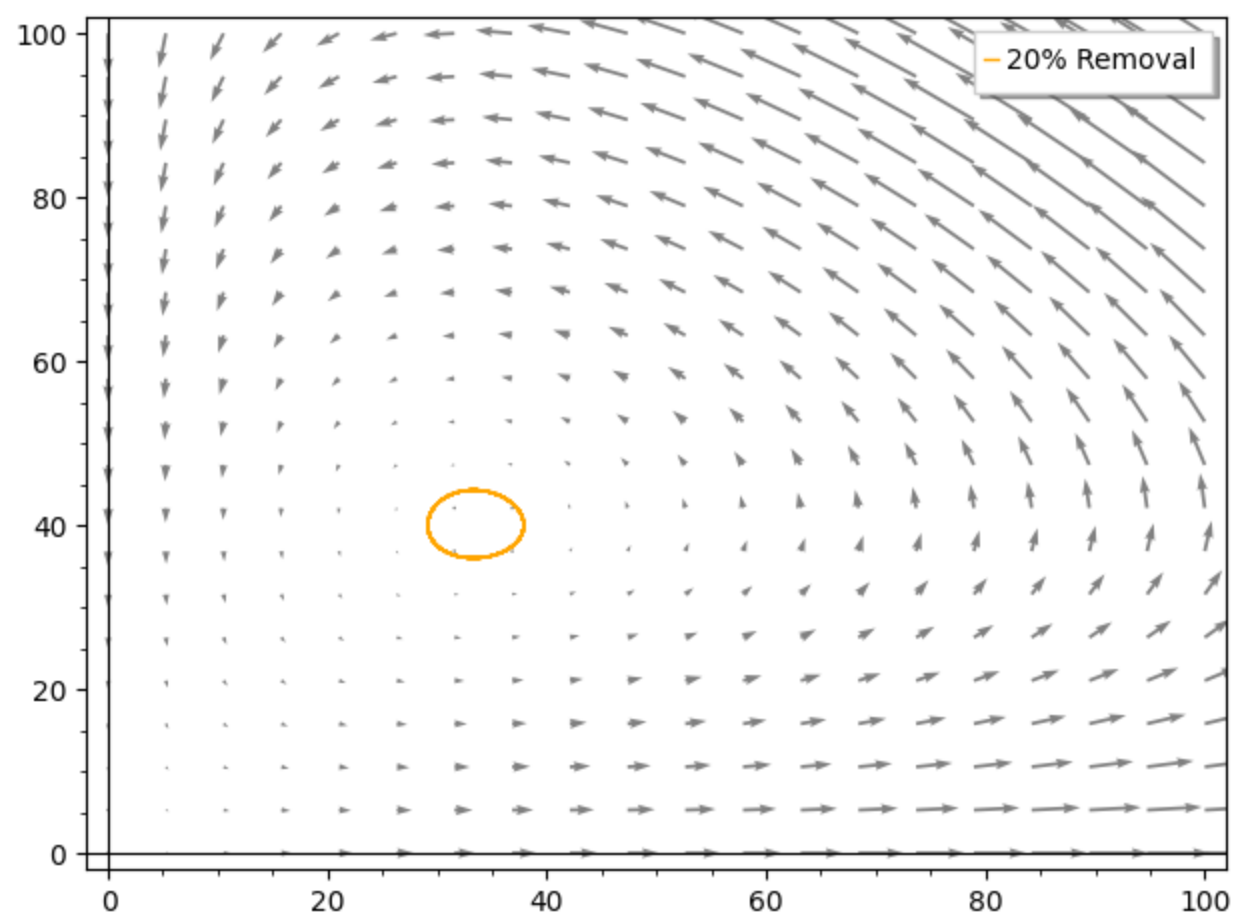
\includegraphics[width=0.5\textwidth]{hw8_3.png}
\item With the same number of predator, 70\% of prey got removed means there are 6 prey left. 

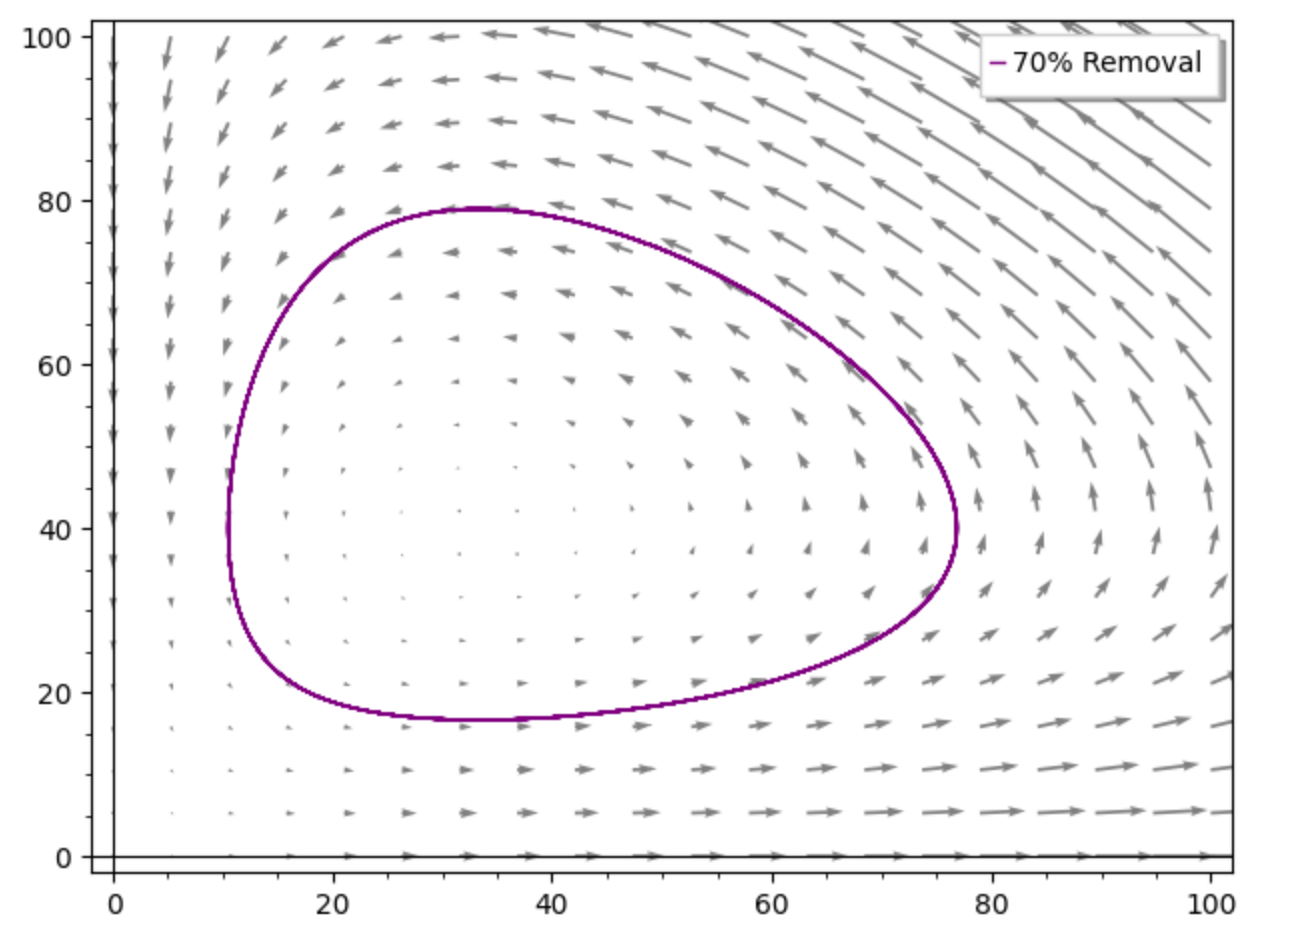
\includegraphics[width=0.5\textwidth]{hw8_4.png}
\item 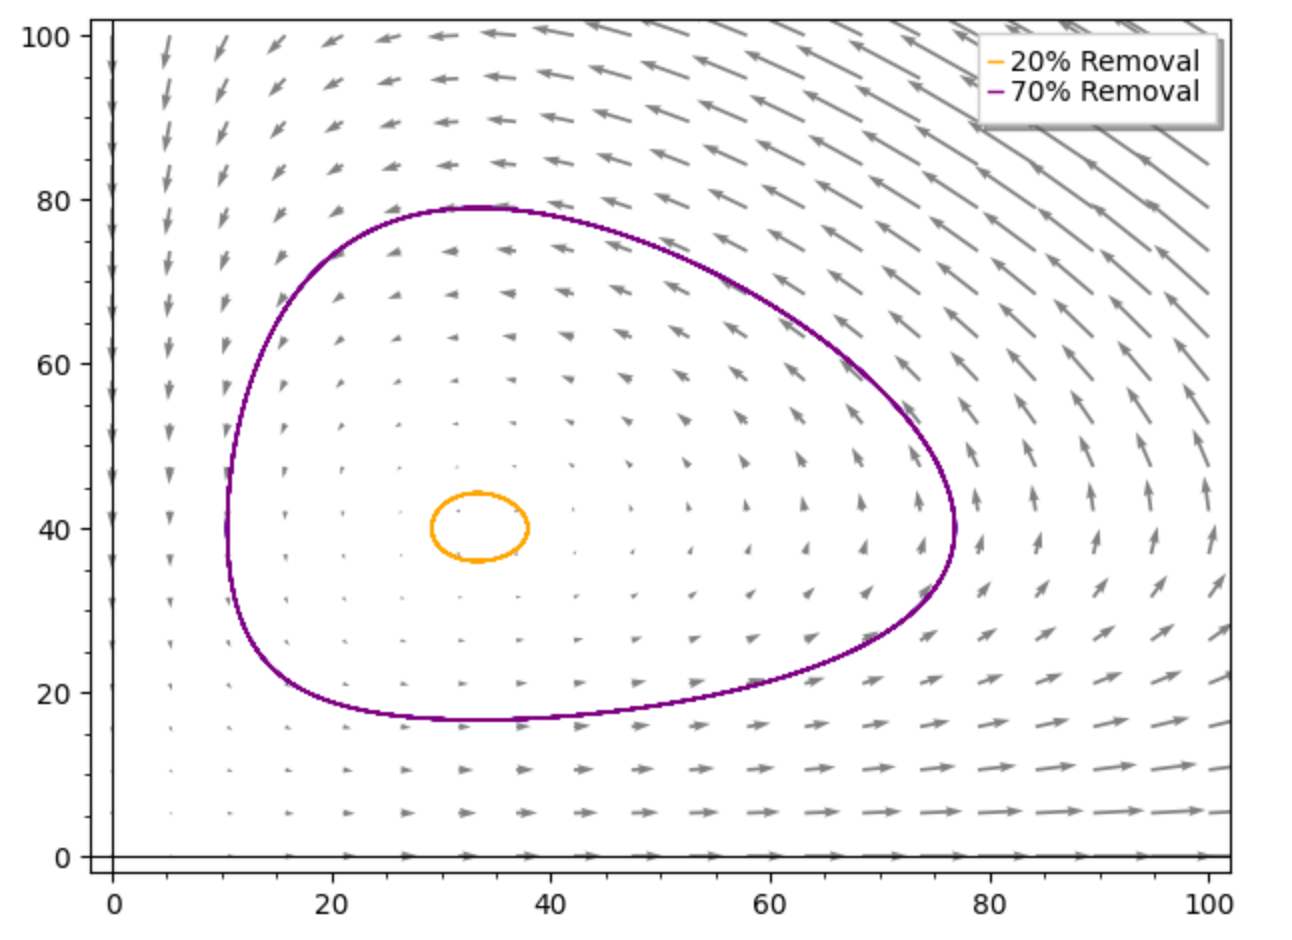
\includegraphics[width=0.5\textwidth]{hw8_5.png}
\item Removing 20\% predators may cause a temporary dip, but the prey population may rebound strongly, leading to another predator surge. But removing 70\% of prey would cause a significant dip in the predator population, which may not recover quickly, leading to a long-term decline in predators.
\end{enumerate}

\section*{\#3.5}
\subsection*{\#1}
If x is strictly equal 0

\subsection*{\#2}
It belongs to the basin of attraction of x = k because the moment it starts there it converges to k.

\subsection*{\#3}
Every time the red and blue lights cross, which is the equilibrium, the concentration changes. With the later part becomes more stable after the second equilibrium, with a longer period of oscillation, based on what I see.

\subsection*{\#4}
It's a saddle point type fo equilibrium? I'm not sure how to answer this one

\section*{Further Excercises 3.5}
\subsection*{\#1}
The event horizon of the black hole, if I understand this correctly, is a representation of the basin of attraction. The moment you step into the event horizon, you are guaranteed to be pulled into the black hole. But if you stay out of it, the law remains the same, represent 2 different equilibrium points.

\subsection*{\#2}
We can define a list of initial conditions across a region of phase space. Then we can simulate trajectories from each initial condition using numerical methods then we observe the long-term behavior, that if the trajectory approaches a particular equilibrium, mark that initial point as belonging to that basin.

\subsection*{\#3}
\begin{figure}[H]
\centering

% One Stable Equilibrium
\begin{minipage}{0.45\textwidth}
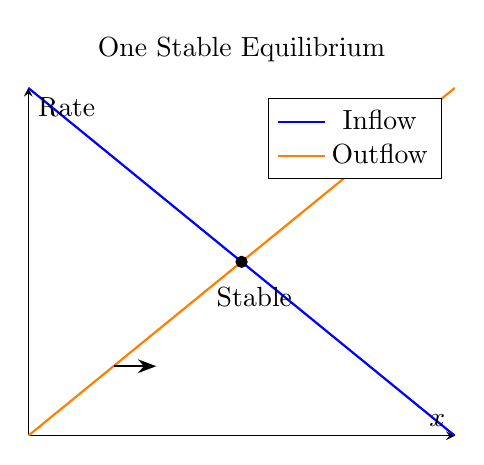
\begin{tikzpicture}[scale=1]
\begin{axis}[
    enlargelimits=false,
    clip=true,
    xtick=\empty, ytick=\empty,
    title={One Stable Equilibrium},
    xlabel={$x$}, ylabel={Rate},
    domain=0:10,
    samples=100,
    axis lines=middle,
    xmin=0, xmax=10, ymin=0, ymax=10,
    legend pos=north east,
    width=7cm, height=6cm,
]
\addplot[blue, thick] {10 - x};
\addplot[orange, thick] {x};
\addlegendentry{Inflow}
\addlegendentry{Outflow}
\addplot[only marks, mark=*] coordinates {(5,5)};
\node at (axis cs:5.3,4) {Stable};

% Arrows
\draw[-{Stealth}, thick] (axis cs:2,2) -- ++(1,0);
\draw[-{Stealth}, thick] (axis cs:8,8) -- ++(-1,0);

\end{axis}
\end{tikzpicture}
\end{minipage}
\captionsetup{belowskip=0pt}

% One Unstable Equilibrium
\begin{minipage}{0.45\textwidth}
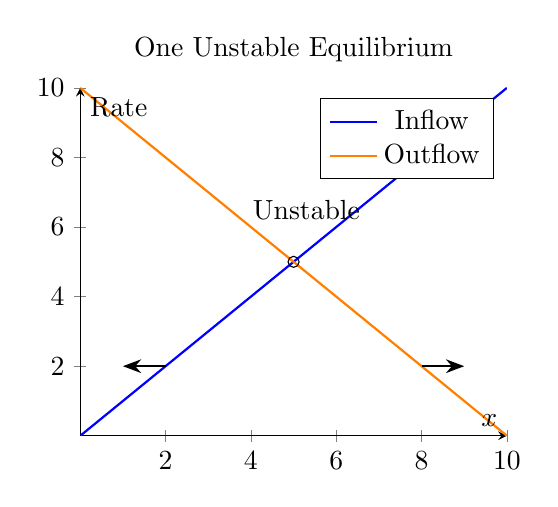
\begin{tikzpicture}[scale=1]
\begin{axis}[
    title={One Unstable Equilibrium},
    xlabel={$x$}, ylabel={Rate},
    domain=0:10,
    samples=100,
    axis lines=middle,
    xmin=0, xmax=10, ymin=0, ymax=10,
    legend pos=north east,
    width=7cm, height=6cm,
]
\addplot[blue, thick] {x};
\addplot[orange, thick] {10 - x};
\addlegendentry{Inflow}
\addlegendentry{Outflow}
\addplot[only marks, mark=o, mark options={fill=white}] coordinates {(5,5)};
\node at (axis cs:5.3,6.5) {Unstable};

% Arrows
\draw[-{Stealth}, thick] (axis cs:2,2) -- ++(-1,0);
\draw[-{Stealth}, thick] (axis cs:8,2) -- ++(1,0);

\end{axis}
\end{tikzpicture}
\end{minipage}

% Three Equilibria
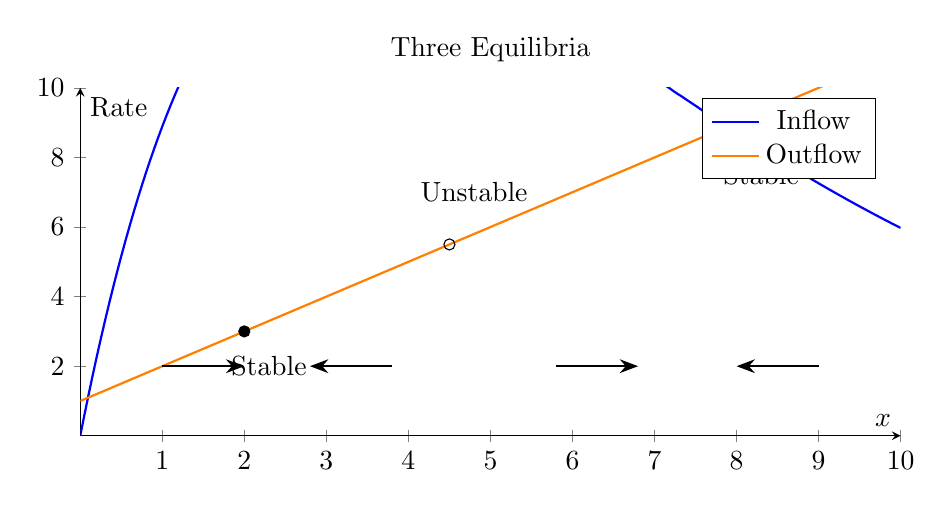
\begin{tikzpicture}[scale=1]
\begin{axis}[
    title={Three Equilibria},
    xlabel={$x$}, ylabel={Rate},
    domain=0:10,
    samples=200,
    axis lines=middle,
    xmin=0, xmax=10, ymin=0, ymax=10,
    legend pos=north east,
    width=12cm, height=6cm,
]
\addplot[blue, thick] {12*x*exp(-0.3*x)};
\addplot[orange, thick] {x + 1};
\addlegendentry{Inflow}
\addlegendentry{Outflow}

% Equilibria (approximate)
\addplot[only marks, mark=*] coordinates {(2,3)};
\addplot[only marks, mark=o, mark options={fill=white}] coordinates {(4.5,5.5)};
\addplot[only marks, mark=*] coordinates {(8,9)};
\node at (axis cs:2.3,2) {Stable};
\node at (axis cs:4.8,7) {Unstable};
\node at (axis cs:8.3,7.5) {Stable};

% Arrows for flow
\draw[-{Stealth}, thick] (axis cs:1,2) -- ++(1,0);
\draw[-{Stealth}, thick] (axis cs:3.8,2) -- ++(-1,0);
\draw[-{Stealth}, thick] (axis cs:5.8,2) -- ++(1,0);
\draw[-{Stealth}, thick] (axis cs:9,2) -- ++(-1,0);

\end{axis}
\end{tikzpicture}

\caption{Inflow and Outflow Curves with Stability Analysis (Over-Under Method)}
\end{figure}

\subsection*{\#4}
\begin{figure}[htbp] % h=here, t=top, b=bottom, p=page of floats
  \centering
  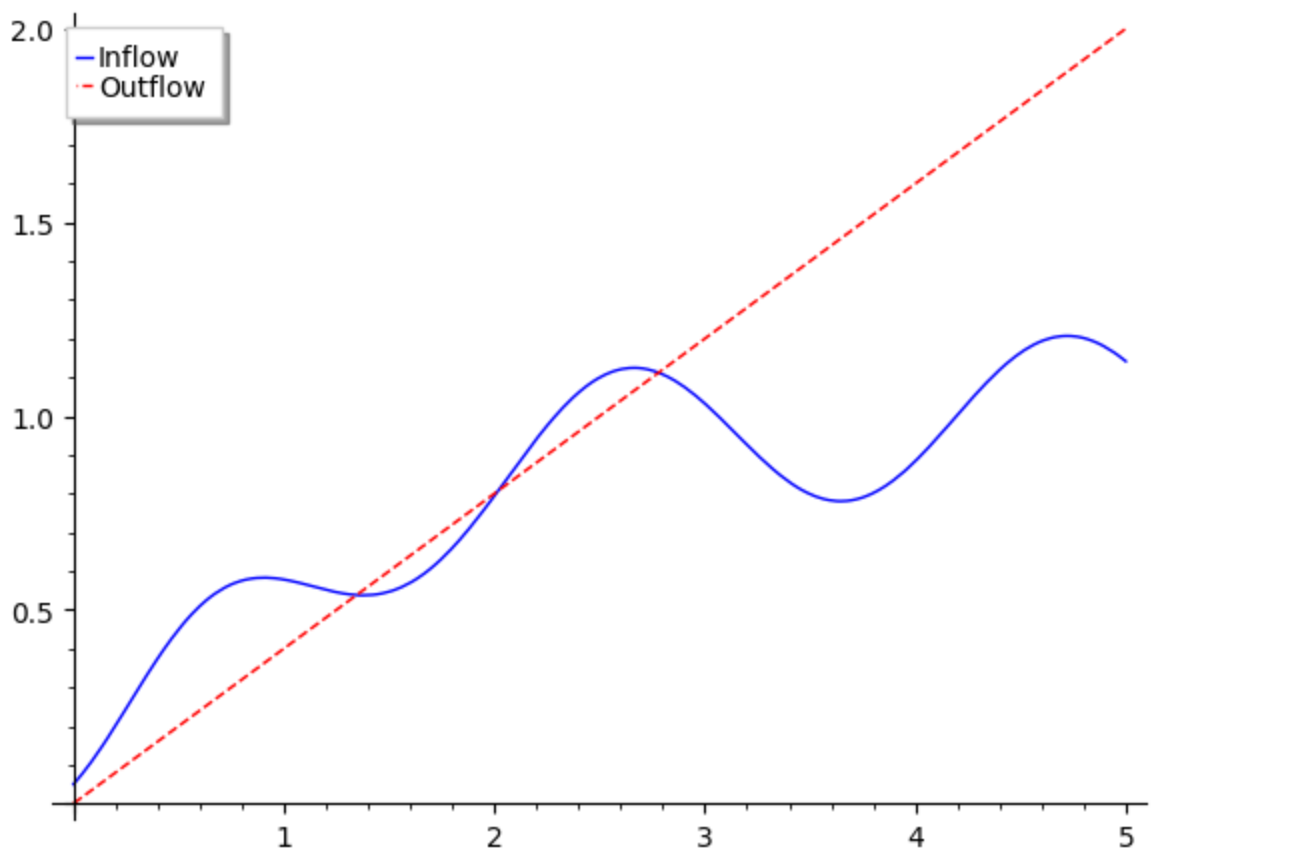
\includegraphics[width=0.6\textwidth]{hw8_6.png}
\end{figure}

\subsection*{\#5}
\begin{figure}[htbp] % h=here, t=top, b=bottom, p=page of floats
  \centering
  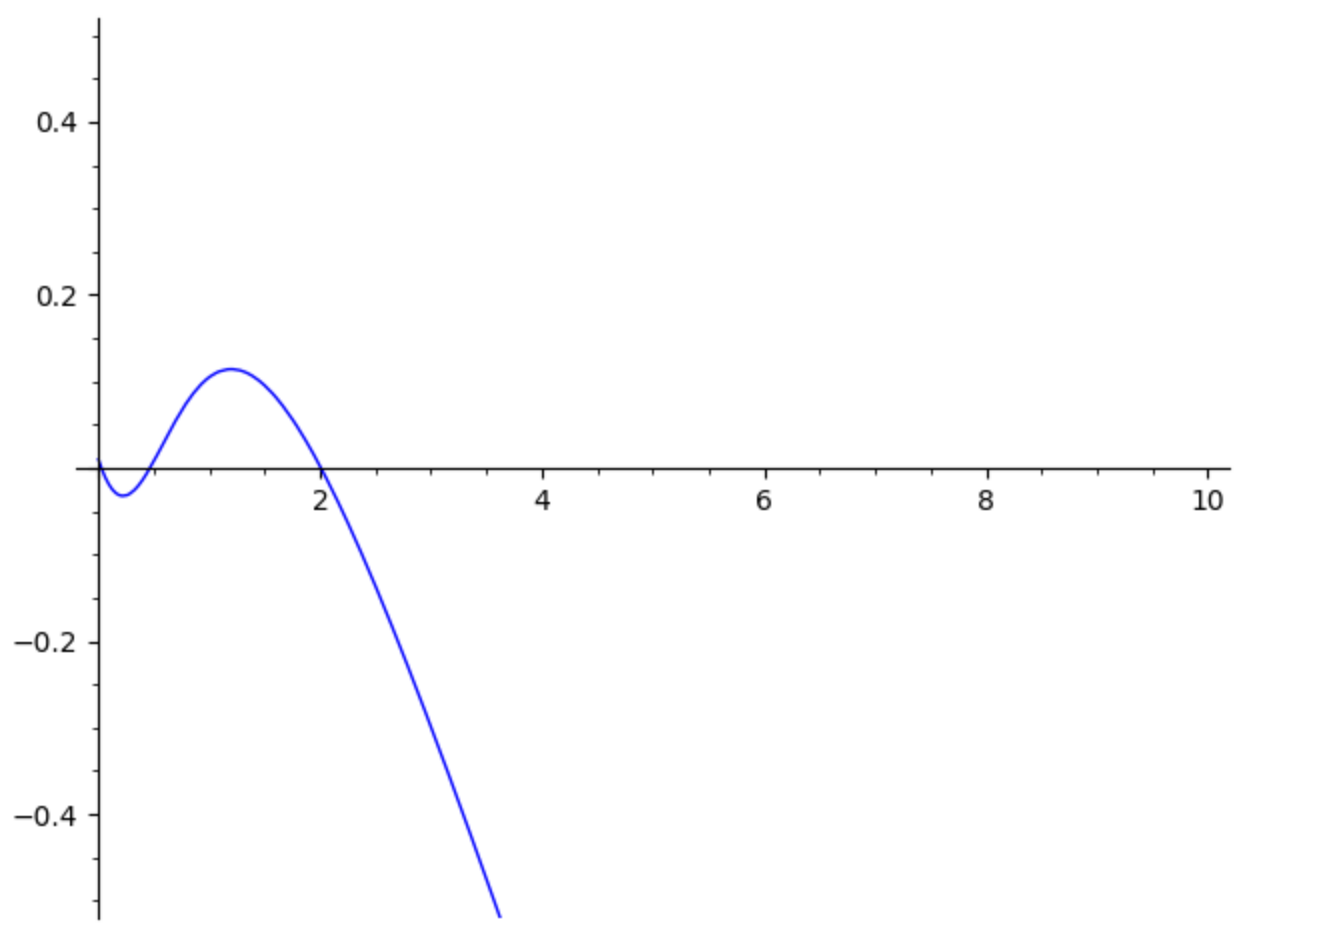
\includegraphics[width=0.6\textwidth]{hw8_7.png}
\end{figure}

There are 2 roots: [0.465, 2.0083] and derivative at these points are:
[0.222419454814250 -0.243030379139503]

I did all in sagemath for convenience
\begin{figure}[htbp] % h=here, t=top, b=bottom, p=page of floats
  \centering
  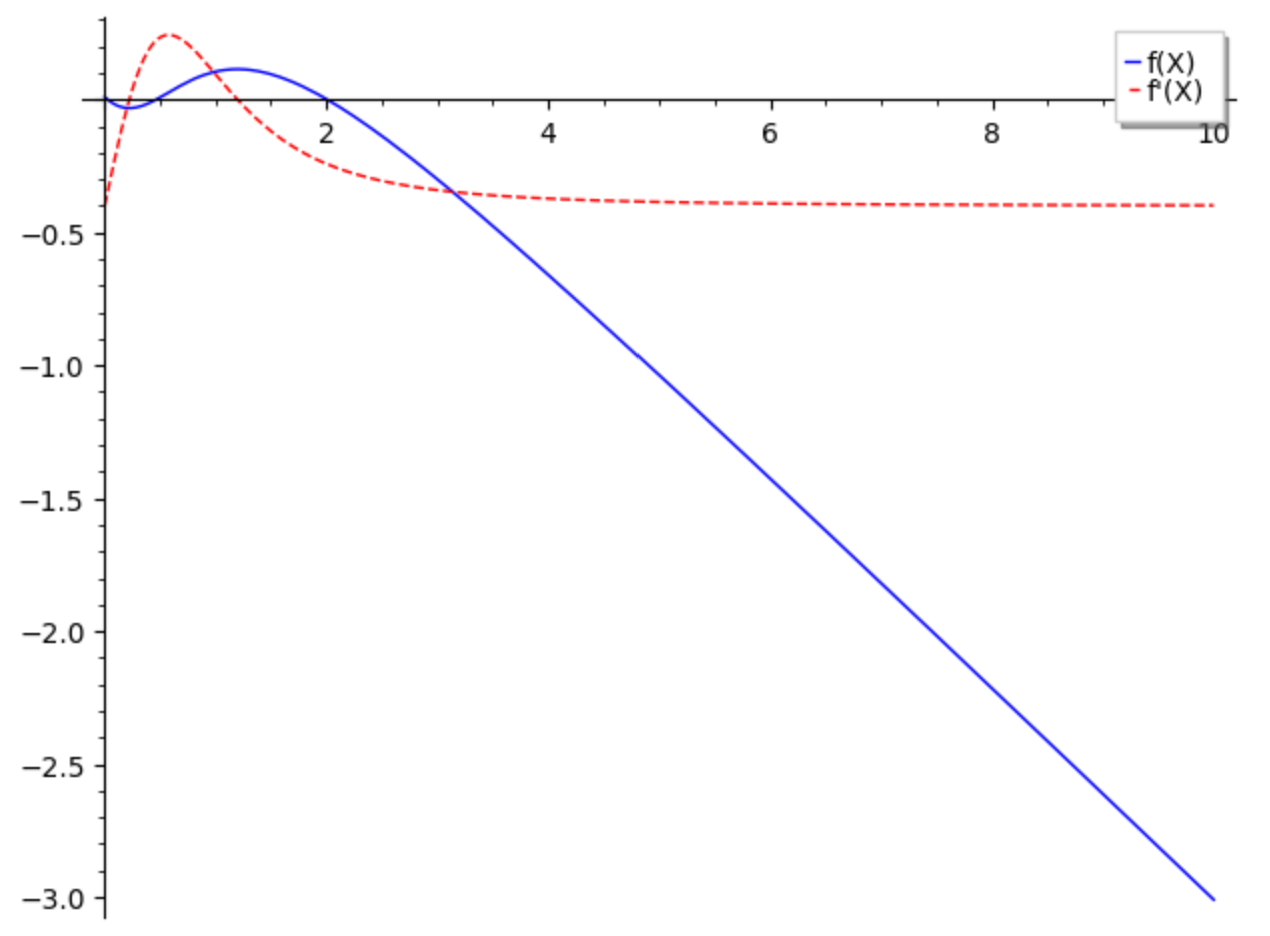
\includegraphics[width=0.6\textwidth]{hw8_8.png}
\end{figure}

\end{document}